\section{Revisão da literatura}\label{sec-revisão}

Nesta seção, serão apresentados trabalhos recuperados da literatura que
dialogam direta ou indiretamente com a temática desenvolvida nesta
pesquisa, sobretudo relacionados aos papéis semânticos em PLN e à
aplicação de SRL.

\subsection{Papéis semânticos nos estudos de PLN}\label{sub-sec-papeissemanticos}

Segundo \textcite{banarescu2013}, o modelo AMR objetiva capturar e
representar explicitamente aspectos do significado de uma sentença. Esse
modelo teórico propõe a enumeração de argumentos na tentativa de
simplificar a proposta de papéis semânticos. \textcite{weischedel2013} apontam que na AMR, tradicionalmente, segue-se a seguinte
proposta:

\begin{itemize}
\item[Arg0]\label{arg0}: refere-se ao argumento da ação que desempenha o papel de agente;
\item[Arg1]\label{arg1}: refere-se ao argumento principal que é afetado pela ação
  expressa pelo verbo, correspondendo, em geral, ao objeto direto;
\item[Arg2]\label{arg2}: refere-se a um argumento secundário ou ao objeto indireto em
  construções que apresentam verbos;
\item[Arg3, Arg4 e Arg5]\label{arg345}: são termos menos frequentes nas construções
  linguísticas, ocorrendo em construções verbais mais complexas, como
  para o verbo ``dar'' ou ``entregar''.
\end{itemize}

A partir dessas definições, é importante ressaltar que a proposta do
modelo AMR pode ou não levar em conta aspectos morfossintáticos e/ou a
ordem em que os itens lexicais ocorrem nas sentenças. O Arg0, por
exemplo, é definido apenas a partir de aspectos semânticos; todos os
outros argumentos levam em conta, em alguma medida, informações
gramaticais que consideram a ordem e/ou a classificação morfossintática.
Outro ponto importante desse modelo é que itens lexicais/\emph{tokens}
que não contribuem fortemente para a construção dos sentidos em
determinadas sentenças (como determinantes/artigos) não são considerados
na análise, dando-se ênfase na estrutura argumental.

A título de exemplificação, tem-se a sentença apresentada em \ref{itm3}, que
foi extraída do \emph{corpus} AMR-PT \cite{inacio2023}, que
contempla sentenças extraídas da obra ``O pequeno príncipe'', dentre
outros gêneros textuais, atualmente.

\begin{enumerate}[start=3,label={(\arabic{enumi})}]
    \item\label{itm3} Meu desenho não representava um chapéu.
\end{enumerate}

De acordo com a proposta AMR, na sentença exemplificada em \ref{itm3}, tem-se
dois argumentos: ``desenho'' é o argumento principal em relação ao verbo
``representar'' e, por isso, recebe a classificação de Arg1; e
``chapéu'', que desempenha o papel de ``objeto'', recebe a classificação
Arg2. Os itens lexicais ``meu'' e ``não'' indicam, respectivamente, a
relação de posse e a polaridade negativa da sentença. Tais relações
também são consideradas e representadas no modelo AMR. Por fim, o item
``um'' não faz parte da estrutura argumental pois não exerce modificação
significativa sobre ``chapéu'', ainda que desempenhe função de
indeterminação sobre ele.

Além disso, o modelo propõe possibilidades de representação do
conhecimento semântico, aspecto extremamente importante para
implementação computacional. Uma dessas representações é a
\emph{estrutura de grafos}, em que os nós representam eventos e
entidades mencionados na sentença; já as arestas representam as relações
entre os nós. A \Cref{fig-01} representa a estrutura argumental do exemplo em \ref{itm3}.

\begin{figure}[h]
  \centering    
  \begin{minipage}{.75\textwidth}
  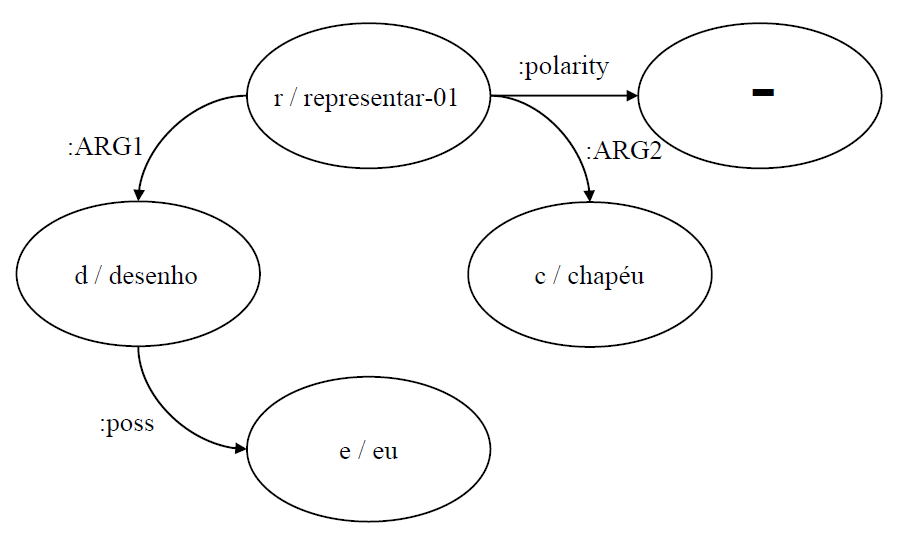
\includegraphics[width=\textwidth]{figure01.png}
  \caption{Exemplo de grafo AMR.}
  \label{fig-01}
  \source{Adaptado de \textcite{anchiêta2022}.}
  \end{minipage}
\end{figure}

Outra possibilidade de representação é por meio de \emph{notação lógica}
(\Cref{fig-02}), em que, a partir da identificação léxica do predicado,
apontam-se os tipos de argumentos, seus respectivos itens lexicais e a
relação semântica estabelecida entre eles. Por fim, na \emph{notação
Penman} (\Cref{fig-03}), feita em formato textual, há delimitação de
instâncias, que são os itens lexicais que funcionam como argumentos e/ou
predicados nas sentenças, a estrutura argumental entre as instâncias e
as relações que podem estabelecer entre si. Cabe destacar que as três
figuras equivalem à mesma representação semântica, sendo que a \Cref{fig-01},
por seu apelo gráfico, pode ser melhor interpretável por humanos, ao
passo que as Figuras 2 e 3 permitem implementações computacionais por
serem notações lógicas.

\begin{figure}[h]
\begin{minipage}{.45\textwidth}
  \centering
  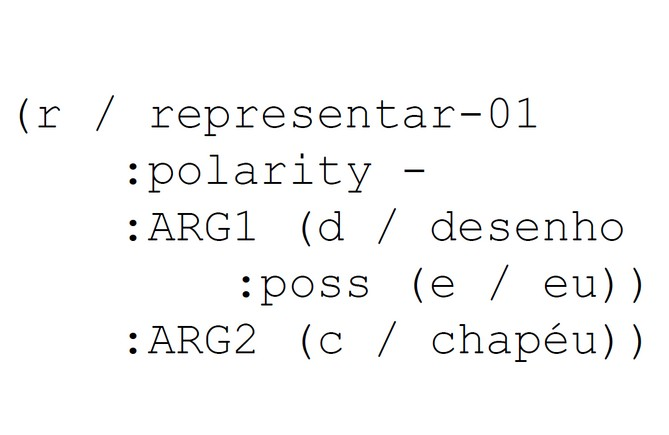
\includegraphics[width=\textwidth]{figure02.jpg}
  \caption{Exemplo de notação lógica no modelo AMR.}
  \label{fig-02}
  \source{Elaborado pelos autores.}
\end{minipage}%
\hfill
\begin{minipage}{.45\textwidth}
  \centering
 
\includegraphics[width=\textwidth]{figure03.jpg}
  \caption{Exemplo de notação Penman no modelo AMR.}
  \label{fig-03}
  \source{Elaborado pelos autores.}
\end{minipage}
\end{figure}

Outro aspecto importante na proposta do modelo é a classificação dos
conceitos. De acordo com \textcite{anchiêta2022}, os conceitos AMR podem
ser classificados em \emph{concretos} (palavras em suas formas
lexicalizadas, como ``mulher'' e ``homem''), \emph{framesets} do
\emph{Proposition Bank} -- PropBank\footnote{PropBank pode ser definido
  como um recurso de sentenças anotadas com funções semânticas
  \cite{jurafsky2023}. Por conta da dificuldade de se obter um
  conjunto ``universal'' de papéis semânticos, como demonstrados nesta
  seção, nos PropBanks convencionou-se que as relações semânticas são
  numeradas (ao invés do uso de seus nomes), que é justamente a
  filosofia adotada pela AMR.} -- \cite{palmer2005} ou
\emph{abstratos} (que não correspondem a nenhuma unidade lexical das sentenças, como ``\%'' e ``endereço de e-mail'', por exemplo).

\subsection{Trabalhos relacionados à SRL}\label{sub-sec-trabalhos}

De acordo com \textcite{hartmann2017}, SRL é uma tarefa em PLN
que detecta eventos descritos em sentenças e os participantes desses
eventos. Os eventos ocorrem nas sentenças sob formas morfológicas de
verbos, nomes, adjetivos e advérbios; porém, a classe que mais é
explorada na literatura é a dos verbos, pois expressam eventos, além de
ser impossível construir orações completas com ausência de verbos. As
demais classes de palavras não expressam eventos da mesma forma que os
verbos, nem em proporção.

Ainda segundo \textcite{hartmann2017}, os métodos empregados na
anotação automática de papéis semânticos são, na maioria, com base em
AM. Nesse contexto, é necessário que haja \emph{corpora} linguísticos
anotados para que os algoritmos de AM possam ser treinados e avaliados
quanto ao desempenho da tarefa a que eles foram submetidos. A literatura
aponta alguns \emph{corpora} disponíveis com anotação AMR, importantes
para as tarefas de SRL, a saber: \textcite{xue2014} para o inglês;
\textcite{vanderwende2015} com uma abordagem multilíngue para
Francês, Alemão, Espanhol e Japonês; \textcite{damonte2019} %\alert{Damonte e Cohen (2018)} 
para as línguas italiana, espanhola, alemã e chinesa; \textcite{migueles2018} especificamente para o espanhol; e \textcite{anchiêta2018} e
\textcite{inacio2023}, para o PB. Destaca-se que há também
recursos com papéis semânticos desvinculados da estruturação completa
proposta pela AMR, como é o caso do PropBank do inglês, citado
anteriormente, e o PropBank.Br \cite{duran2012} e o recente PBP
(\emph{Porttinari-base Propbank}) para o português \cite{freitas2024}.

Em especial, o \emph{corpus} para o PB é composto por sentenças anotadas
com o modelo AMR para diferentes gêneros textuais. A primeira versão do
\emph{corpus} apresentava sentenças extraídas do romance ``O pequeno
príncipe'', tido como \emph{corpus} ``\emph{little prince}''. Em sua
segunda versão, o escopo de domínio foi ampliado para notícias extraídas
do jornal Folha de S. Paulo \cite{duran2012}, tido como o
\emph{corpus} ``\emph{news}''. Em sua versão mais recente\footnote{Disponível
  em: \href{https://github.com/nilc-nlp/AMR-BP}{GitHub -
  nilc-nlp/AMR-BP}. Acesso em: 20 jul.2024.}, o AMR-PB apresenta textos
opinativos, tido como \emph{corpus} ``\emph{opisums}'', e científicos,
tido como \emph{corpus} ``\emph{sci}''. Ademais, todos os \emph{corpora}
apresentam sentenças anotadas, identificando os papéis semânticos
seguindo a metodologia do PropBank.Br \cite{duran2012}.

Com relação ao PropBank.Br, \textcite{duran2012} destacam que o
\emph{corpus} é um repositório de proposições, alinhando-se ao que
\textcite{fillmore1968} apresenta sobre a estrutura base de uma frase, a saber:
um conjunto de relações entre substantivos e verbos, sem modificadores
de tempo, negação, aspecto e modo. Segundo as autoras, os verbos recebem
um código que indica seu sentido com relação ao \emph{frame} em que a
sentença está associada; já os argumentos são anotados com rótulos de
função numerados (de Arg0 a Arg5) e os modificadores são anotados com
rótulos de função ArgMs (Modificadores de argumento).

Vale a pena ressaltar que os \emph{corpora} delimitados aqui seguem as
diretrizes da literatura quanto ao PLN. Os conjuntos de dados
linguísticos acompanham os apontamentos de \textcite{gildea2002}, já
que representam semanticamente os papéis temáticos distanciando-se de
detalhamentos analíticos, ao passo que se aproximam da objetividade e
simplificação de rótulos para garantir melhor desempenho no processo de
classificação automática.

Partindo de \emph{corpora} anotados, é possível aplicar diferentes
técnicas de AM. O trabalho de \textcite{hartmann2015} realizou a análise
automática de papéis semânticos utilizando AM nos \emph{subcorpora news}
e \emph{opisums}. Aplicando diferentes abordagens (utilizando ou não
árvores sintáticas treinadas), os autores obtiveram Medida-F de 87,8\%
para o \emph{corpus news}, e 94,5\% para o \emph{corpus opisums}.

Hartmann, \textcite{duran2012} realizaram a avaliação de dois sistemas
de SRL para textos jornalísticos. O sistema desenvolvido por \textcite{fonseca2013} teve o propósito de anotar automaticamente os papéis
semânticos para o PB, sem lançar mão de ferramentas de PLN externas ao
sistema desenvolvido; os resultados dessa avaliação indicam uma Medida-F
de 68\%. Já o sistema de \textcite{alva-manchego2012} empregou a abordagem
supervisionada de AM e obteve Medida-F de 79,6\%. Destaca-se que ambos
os trabalhos foram baseados no \emph{corpus} PropBank.Br.

\textcite{ilmy2021} realizaram a análise de frases em indonésio
utilizando a AMR com abordagem de aprendizado de máquina. Inspirado no
trabalho de \textcite{zhang2019}, o sistema desenvolvido por \textcite{ilmy2021} compreende três etapas: (i) previsão de pares de palavras, (ii)
previsão de rótulos e (iii) construção de grafos. Em (i), utiliza-se um
componente de análise de dependência para obter as conexões entre
palavras. Em (ii), emprega-se um algoritmo de aprendizado supervisionado
para prever os rótulos entre as conexões. Em (iii), a partir dos rótulos
previstos, é criado o grafo da sentença em AMR. Avaliado com uma base de
dados de frases simples coletadas de artigos e notícias, o modelo
atingiu uma pontuação SMATCH\footnote{SMATCH é uma métrica que tem como
  objetivo avaliar estruturas semânticas em ocorrências linguísticas
  \cite{cai2013}.} de 0,820.
